\documentclass[column,brazilian,12pt,a4paper,final]{article}
\usepackage[brazil]{babel}
%\usepackage{nonfloat}
\usepackage[utf8]{inputenc}
\usepackage{multicol}
\usepackage{hyperref}
\usepackage[pdftex]{color,graphicx}
\usepackage{geometry}
\usepackage{amsmath}
\usepackage{caption}

 \geometry{
 a4paper,
 total={170mm,257mm},
 left=20mm,
 top=20mm,
 }
 \usepackage{ragged2e}
\usepackage{fancyhdr}
\usepackage{caption}[=v1]
\usepackage{xcolor}
\usepackage{circuitikz}
\pagestyle{plain}
\fancyhead{}
\lhead{
\includegraphics[width=1.5cm]{logoufrgs}}
\rhead{
\includegraphics[width=0.8cm]{logoif}}
\fancyfoot{}
\fancyhead[C]{\footnotesize Física Experimental III $\bullet$ 2025/1}
\fancyfoot[RO]{\thepage}
\usepackage{float}
\usepackage{setspace}
\usepackage{fancyref}


\title{}
\author{Autores: \\ Lucas Assis Paulino da Silva - 590174 \\Lucas Bertazo de Deus Félix - 587064
 \\ Pedro Henrique Reis de Oliveira - 590908 \\ IF-UFRGS}
\date{Abril 2025}

\begin{document}
\maketitle
\thispagestyle{fancy}

\section*{Resumo}
\paragraph{}
[...]

\section{Introdução}
\paragraph{}
[...]

\section{Embasamento Teórico}
\paragraph{}
[...]

\section{Material Utilizado}
\begin{itemize}
    \item Fios, conectores, circuito
    \item Multímetro Minipa® ET-2075B (Precisão 0,001V e 0,01$\mu$F)
    \item Fonte Elétrica - IF UFRGS
    \item Capacitor (23,28$\mu$F)
    \item Cronômetro (Precisão 0,01s)
    \item Smartphone com câmera (Para gravação do vídeo)
\end{itemize}

\section{Procedimentos e Montagem}
\paragraph{}
[...]

\section{Dados Experimentais}
\paragraph{}
Os dados de tensão ($V$) em função do tempo ($t$) foram adquiridos com o auxílio de um osciloscópio. Para garantir a reprodutibilidade e avaliar a consistência dos resultados, registramos pelo menos 10 medições para cada um dos três cenários experimentais definidos: com a bobina geradora e o ímã, com a bobina geradora e a bobina detectora, sem o núcleo de ferro na geradora e por último com a bobina geradora e a bobina detectora, com a inserção do núcleo de ferro na geradora.

A seguir, apresentamos um gráfico representativo de cada cenário. Para facilitar a visualização do evento de indução, os gráficos foram plotados no intervalo de tempo específico onde o pulso de tensão ocorre. A análise quantitativa subsequente focará na determinação do fluxo a partir da integral da curva V(t). O conjunto completo de dados brutos para todas as medições pode ser consultado no Apêndice.

\begin{figure}[H]
    \centering
    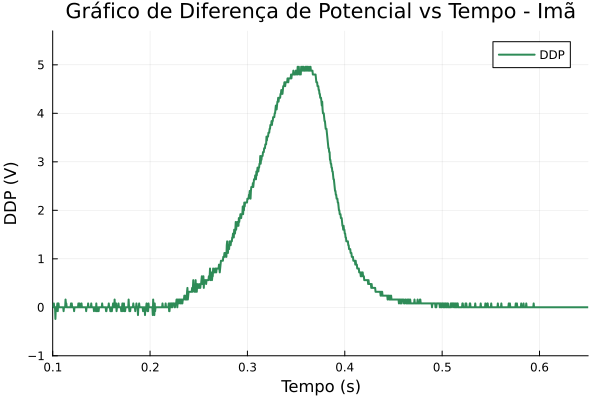
\includegraphics[width=0.75\textwidth]{figuras/grafico_diferenca_potencial - 1.png}
    \caption{Gráfico de tensão versus tempo com a bobina geradora e o imã.}
    \label{fig:grafico1}
\end{figure}
\begin{figure}[H]
    \centering
    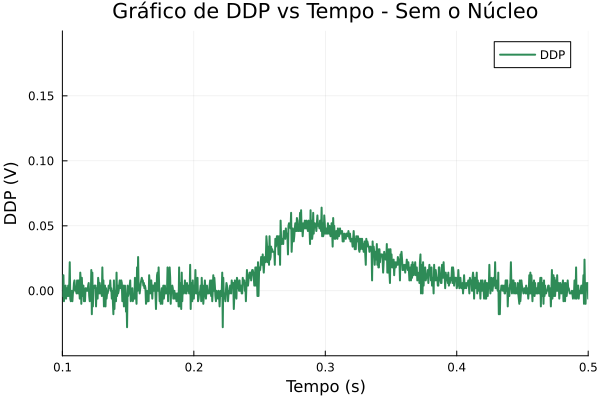
\includegraphics[width=0.75\textwidth]{figuras/grafico_diferenca_potencial - 2.png}
    \caption{Gráfico de tensão versus tempo com a bobina geradora e o detector sem o núcleo de ferro.}
    \label{fig:grafico2}
\end{figure}
\begin{figure}[H]
    \centering
    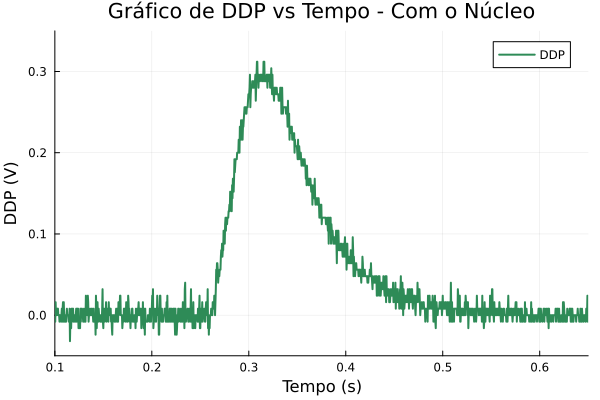
\includegraphics[width=0.8\textwidth]{figuras/grafico_diferenca_potencial - 3.png}
    \caption{Gráfico de tensão versus tempo com a bobina geradora e o detector com o núcleo de ferro.}
    \label{fig:grafico3}
\end{figure}



\section{Análise de Dados}
\paragraph{}
De posse dos dados experimentais, utilizamos a integração numérica pelo método do trapézio para analisar a relação entre a tensão induzida e o fluxo magnético. Conforme a Lei de Faraday, mais especificamente utilizando a relação expressa na equação (14), a integral da tensão em função do tempo está diretamente ligada à variação total do fluxo magnético através da bobina detectora. O resultado esperado é que o valor desta integral, $\int V(t)dt$, seja constante para todas as medições realizadas sob o mesmo cenário experimental. A justificativa para essa constância é que a variação total do fluxo magnético depende apenas das configurações inicial e final do sistema, que são as mesmas em cada repetição do experimento. As pequenas flutuações observadas entre os valores medidos são atribuídas às incertezas experimentais do procedimento.\\

Os resultados obtidos para o fluxo magnético e campo magnético são apresentados na tabela a seguir. A tabela inclui os valores médios e os desvios padrão, calculados a partir das medições realizadas.
\begin{table}[H]
    \centering
    \begin{tabular}{|c|c|c|c|}
        \hline
        Gerador do Campo $B$ & Fluxo Magnético ($\Phi$) & Desvio Padrão ($\sigma$)& Campo Magnético ($B$) \\
        \hline
        Ímã & $9,58.10^{-5}$ Wb &  $3,89.10^{-7}$ & $3,83.10^{-2}$ T \\
        Bobina geradora & $2,71.10^{-8}$ Wb & $9,34.10^{-10}$ & $1,08.10^{-5}$ T \\
        Eletroimã & $5,60.10^{-7}$ Wb & $1,65.10^{-8}$ & $2,24.10^{-4}$ T \\
        \hline
    \end{tabular}
    \caption{Resultados dos fluxos magnéticos e campos magnéticos para os diferentes cenários experimentais.}
    \label{tab:resultados_fluxo_campo}
\end{table}

Usando os valores encontrados, e a propagação de incertezas, obtemos um valor para a constante de permeabilidade magnética do material do núcleo de ferro, $\mu$, que é calculada pela relação $\mu = \frac{B_{Nucleo}}{B_{Sem Nucleo}} . \mu_0$, igual a:
\begin{equation}
    2,60.10^{-5} \pm 4.71.10^{-7} \frac{T.m}{A}. 
\end{equation}
Esse valor é plausível, pois está na ordem de grandeza esperada para materiais compostos de ferro com impurezas.

\section{Conclusão}
[...]

\begin{thebibliography}{99}

\bibitem{}
Processamento de dados e produção de gráficos:
\url{https://github.com/pedro-hro/Relatorio_3-ExperimentalIII}
\bibitem{}
RUTH W. CHABBAY. Matter and Interactions 4th Edition - Matter and Interactions, 4th Edition. WILEY, 2015.
\bibitem{}
NUSSENZVEIG, H. Moysés. {\em Curso de Física Básica - Mecânica}. 5ª ed., vol. 3. São Paulo: Edgard Blücher Ltda, 2013.
\bibitem{}
Schechner, S. J. (2015). The Art of Making Leyden Jars and Batteries according to Benjamin Franklin. ERittenhouse, 26. https://saraschechner.scholars.harvard.edu/publications/art-making-leyden-jars-and-batteries-according-benjamin-franklin


\end{thebibliography}

%\section*{Apêndice - Gráficos de DDP vs Tempo}
\section*{Gráficos de DDP vs Tempo}
\begin{center}
\begin{multicols}{2}

\begin{figure}[H]
    \centering
    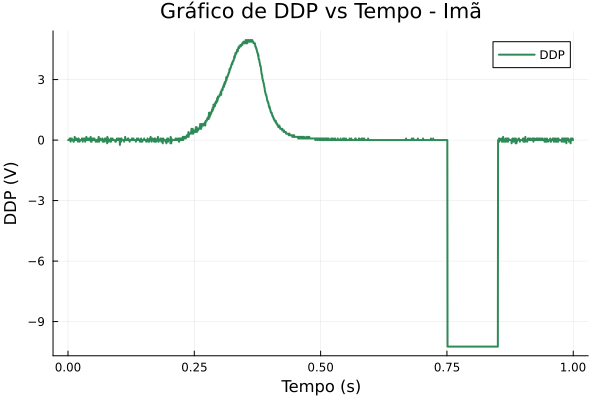
\includegraphics[width=1.0\linewidth]{figuras/grafico_dados1_F0002CH1.png}
\end{figure}

\begin{figure}[H]
    \centering
    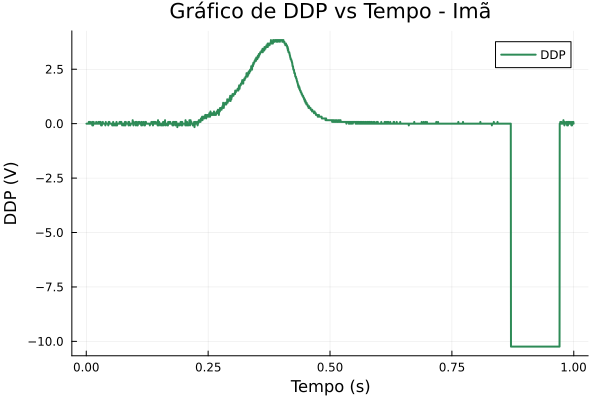
\includegraphics[width=1.0\linewidth]{figuras/grafico_dados1_F0003CH1.png}
\end{figure}

\begin{figure}[H]
    \centering
    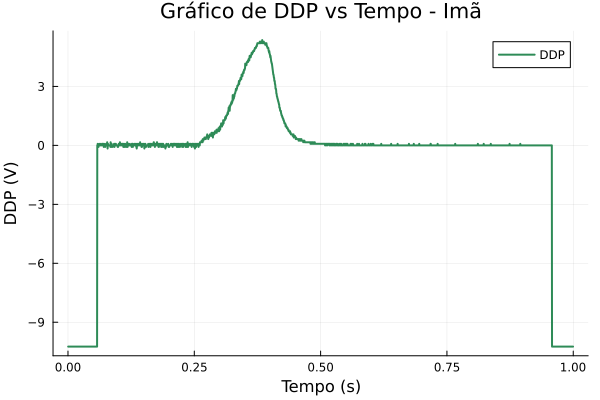
\includegraphics[width=1.0\linewidth]{figuras/grafico_dados1_F0004CH1.png}
\end{figure}

\begin{figure}[H]
    \centering
    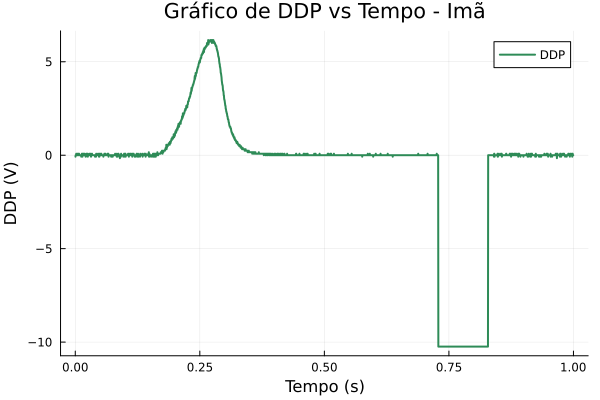
\includegraphics[width=1.0\linewidth]{figuras/grafico_dados1_F0005CH1.png}
\end{figure}

\begin{figure}[H]
    \centering
    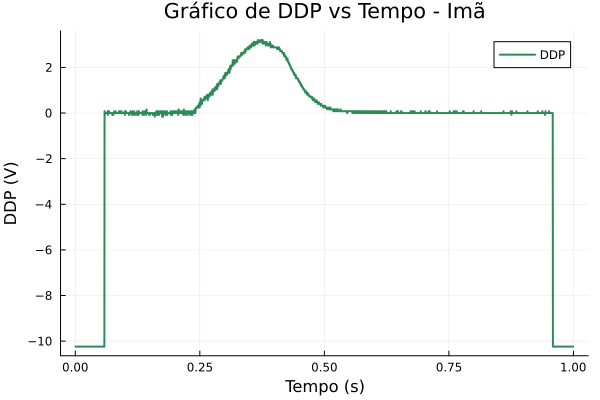
\includegraphics[width=1.0\linewidth]{figuras/grafico_dados1_F0006CH1.png}
\end{figure}

\begin{figure}[H]
    \centering
    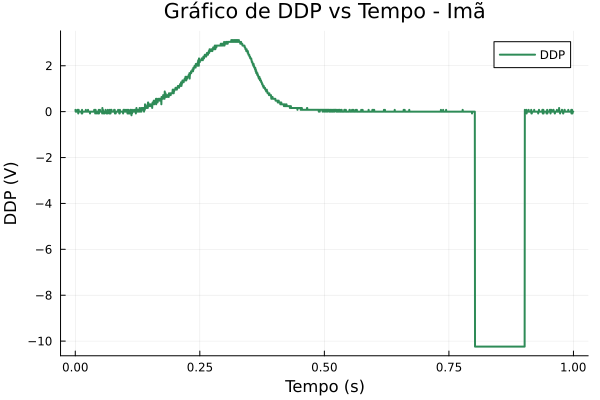
\includegraphics[width=1.0\linewidth]{figuras/grafico_dados1_F0007CH1.png}
\end{figure}

\begin{figure}[H]
    \centering
    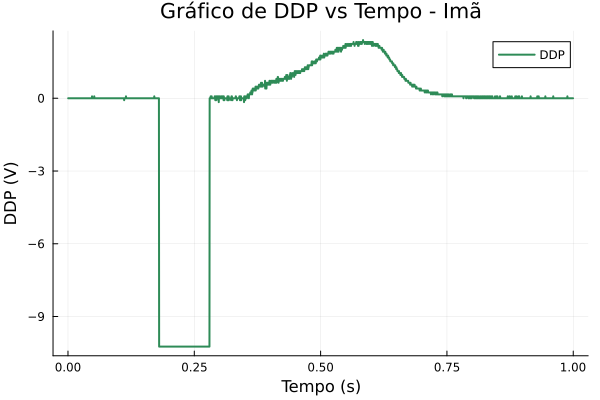
\includegraphics[width=1.0\linewidth]{figuras/grafico_dados1_F0008CH1.png}
\end{figure}

\begin{figure}[H]
    \centering
    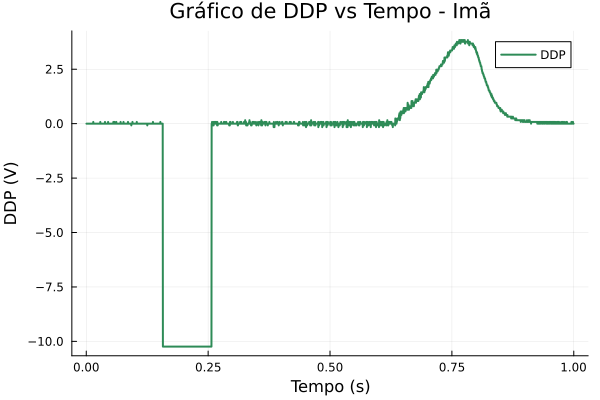
\includegraphics[width=1.0\linewidth]{figuras/grafico_dados1_F0009CH1.png}
\end{figure}

\begin{figure}[H]
    \centering
    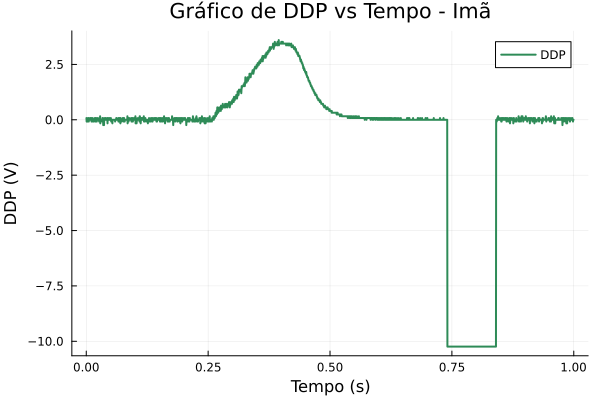
\includegraphics[width=1.0\linewidth]{figuras/grafico_dados1_F0010CH1.png}
\end{figure}

\begin{figure}[H]
    \centering
    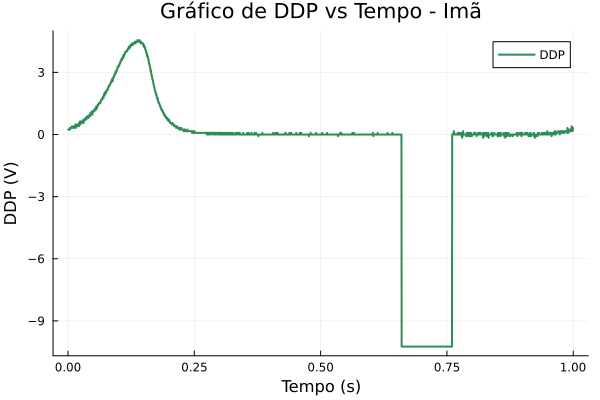
\includegraphics[width=1.0\linewidth]{figuras/grafico_dados1_F0011CH1.png}
\end{figure}

\begin{figure}[H]
    \centering
    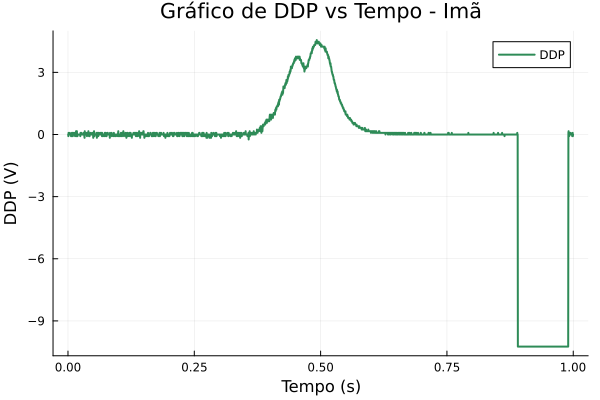
\includegraphics[width=1.0\linewidth]{figuras/grafico_dados1_F0012CH1.png}
\end{figure}

\begin{figure}[H]
    \centering
    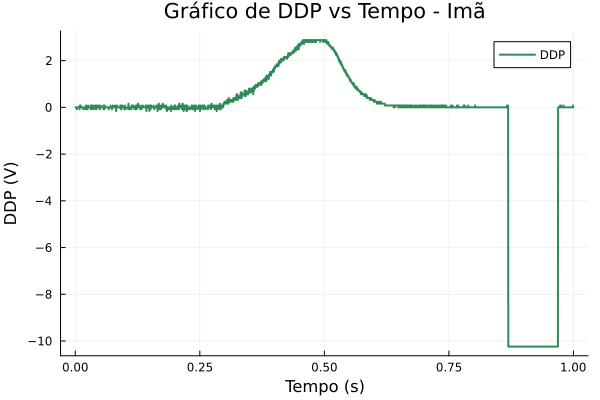
\includegraphics[width=1.0\linewidth]{figuras/grafico_dados1_F0013CH1.png}
\end{figure}

\begin{figure}[H]
    \centering
    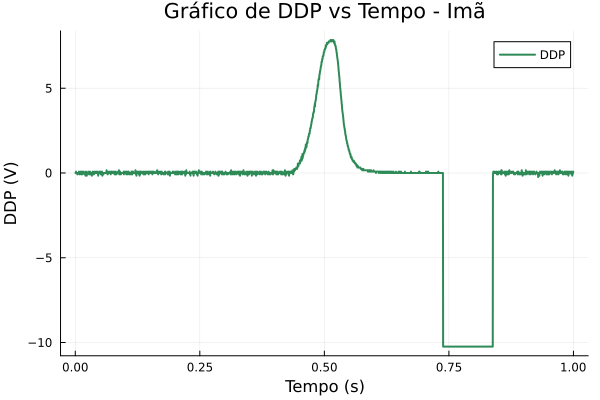
\includegraphics[width=1.0\linewidth]{figuras/grafico_dados1_F0014CH1.png}
\end{figure}

\begin{figure}[H]
    \centering
    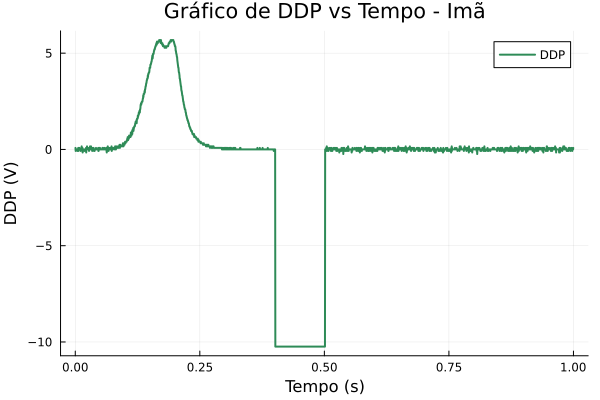
\includegraphics[width=1.0\linewidth]{figuras/grafico_dados1_F0016CH1.png}
\end{figure}

\begin{figure}[H]
    \centering
    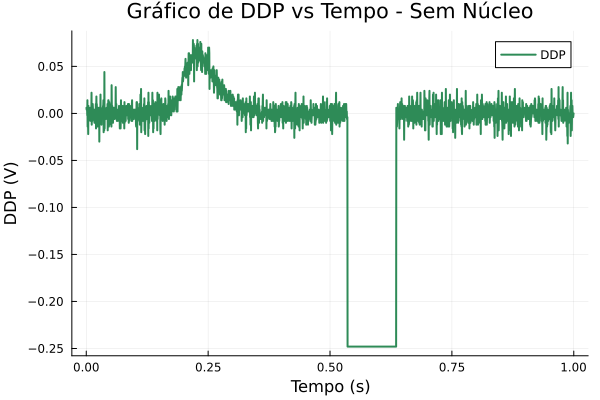
\includegraphics[width=1.0\linewidth]{figuras/grafico_dados2_F0000CH1.png}
\end{figure}

\begin{figure}[H]
    \centering
    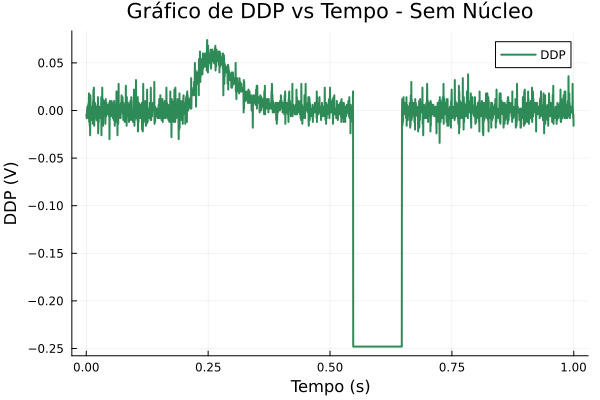
\includegraphics[width=1.0\linewidth]{figuras/grafico_dados2_F0001CH1.png}
\end{figure}

\begin{figure}[H]
    \centering
    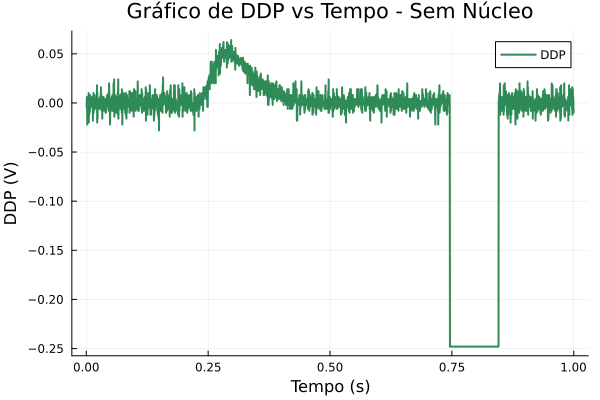
\includegraphics[width=1.0\linewidth]{figuras/grafico_dados2_F0002CH1.png}
\end{figure}

\begin{figure}[H]
    \centering
    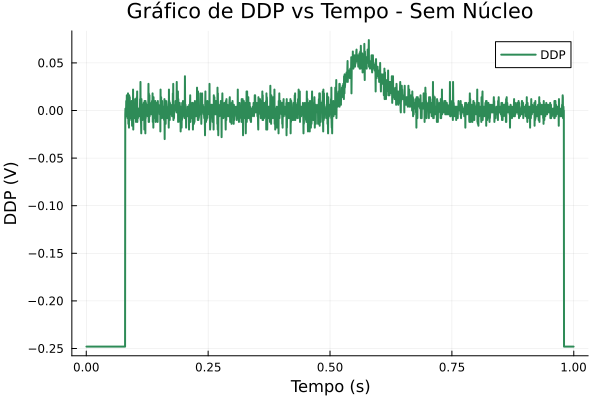
\includegraphics[width=1.0\linewidth]{figuras/grafico_dados2_F0003CH1.png}
\end{figure}

\begin{figure}[H]
    \centering
    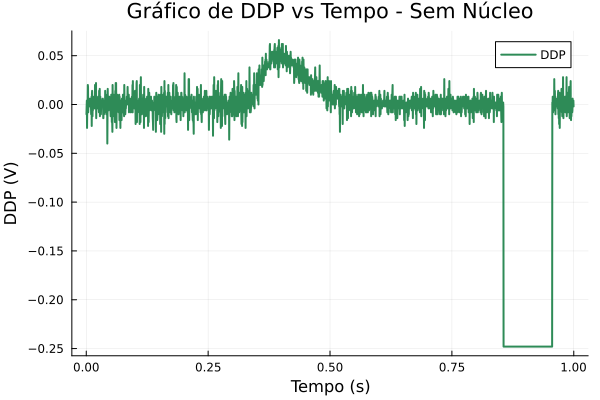
\includegraphics[width=1.0\linewidth]{figuras/grafico_dados2_F0004CH1.png}
\end{figure}

\begin{figure}[H]
    \centering
    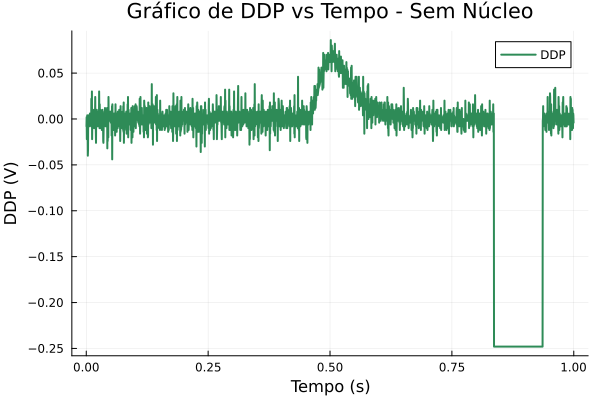
\includegraphics[width=1.0\linewidth]{figuras/grafico_dados2_F0005CH1.png}
\end{figure}

\begin{figure}[H]
    \centering
    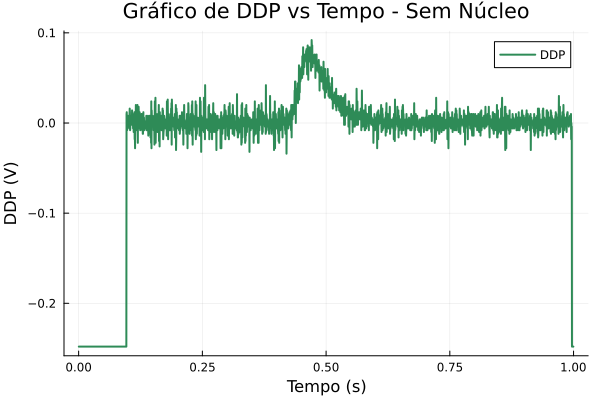
\includegraphics[width=1.0\linewidth]{figuras/grafico_dados2_F0006CH1.png}
\end{figure}

\begin{figure}[H]
    \centering
    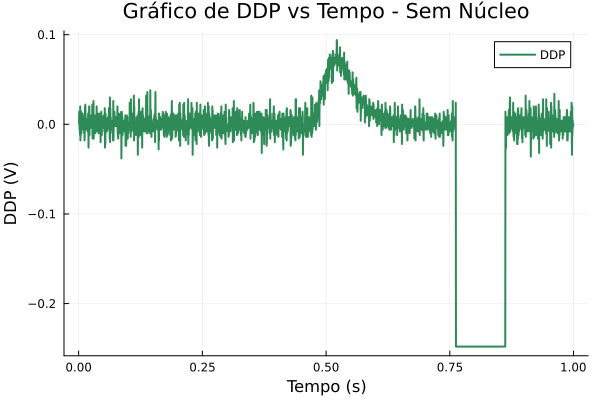
\includegraphics[width=1.0\linewidth]{figuras/grafico_dados2_F0007CH1.png}
\end{figure}

\begin{figure}[H]
    \centering
    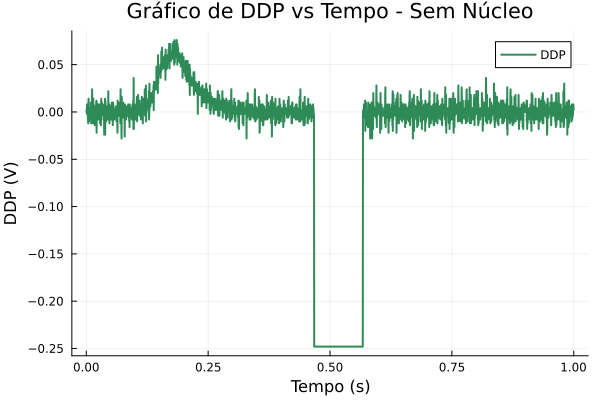
\includegraphics[width=1.0\linewidth]{figuras/grafico_dados2_F0008CH1.png}
\end{figure}

\begin{figure}[H]
    \centering
    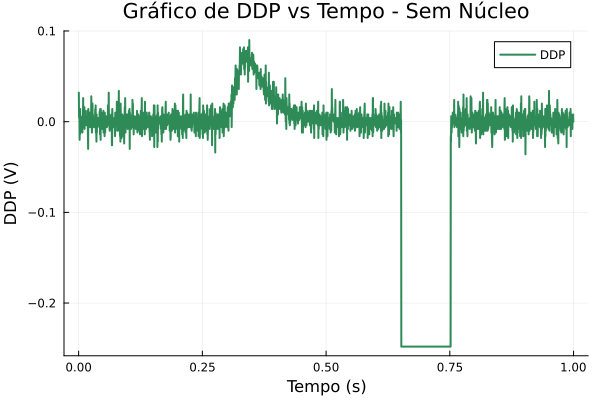
\includegraphics[width=1.0\linewidth]{figuras/grafico_dados2_F0009CH1.png}
\end{figure}

\begin{figure}[H]
    \centering
    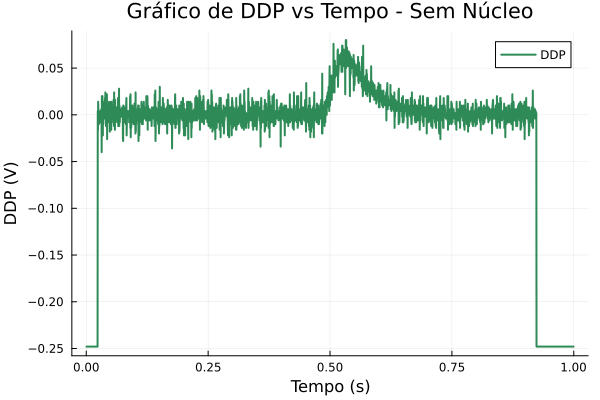
\includegraphics[width=1.0\linewidth]{figuras/grafico_dados2_F0010CH1.png}
\end{figure}

\begin{figure}[H]
    \centering
    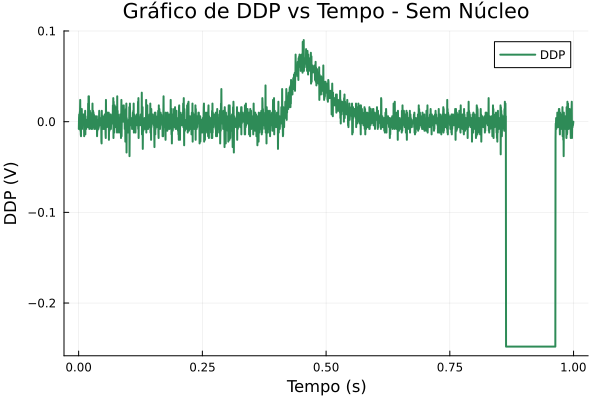
\includegraphics[width=1.0\linewidth]{figuras/grafico_dados2_F0011CH1.png}
\end{figure}

\begin{figure}[H]
    \centering
    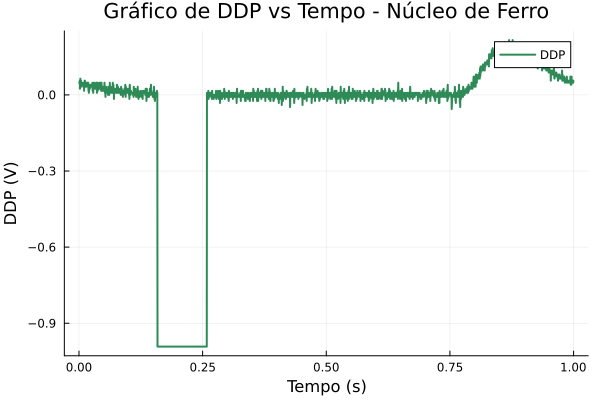
\includegraphics[width=1.0\linewidth]{figuras/grafico_dados3_F0000CH1.png}
\end{figure}

\begin{figure}[H]
    \centering
    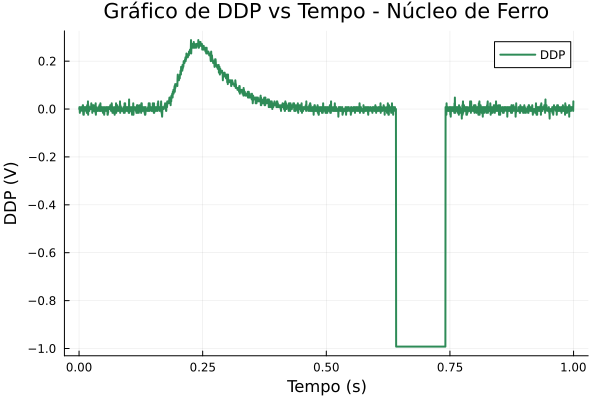
\includegraphics[width=1.0\linewidth]{figuras/grafico_dados3_F0001CH1.png}
\end{figure}

\begin{figure}[H]
    \centering
    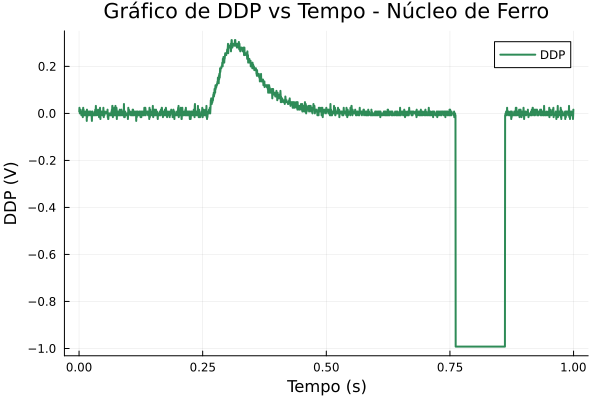
\includegraphics[width=1.0\linewidth]{figuras/grafico_dados3_F0002CH1.png}
\end{figure}

\begin{figure}[H]
    \centering
    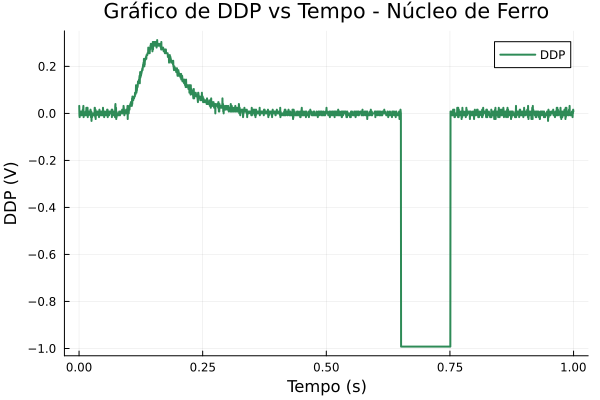
\includegraphics[width=1.0\linewidth]{figuras/grafico_dados3_F0003CH1.png}
\end{figure}

\begin{figure}[H]
    \centering
    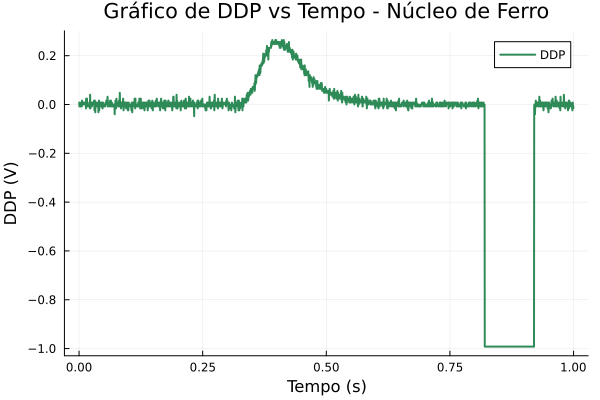
\includegraphics[width=1.0\linewidth]{figuras/grafico_dados3_F0004CH1.png}
\end{figure}

\begin{figure}[H]
    \centering
    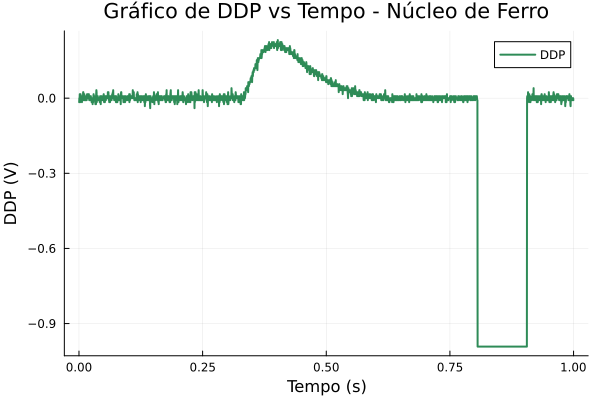
\includegraphics[width=1.0\linewidth]{figuras/grafico_dados3_F0005CH1.png}
\end{figure}

\begin{figure}[H]
    \centering
    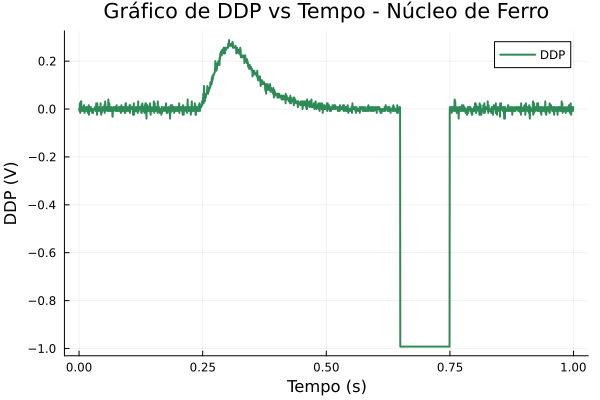
\includegraphics[width=1.0\linewidth]{figuras/grafico_dados3_F0006CH1.png}
\end{figure}

\begin{figure}[H]
    \centering
    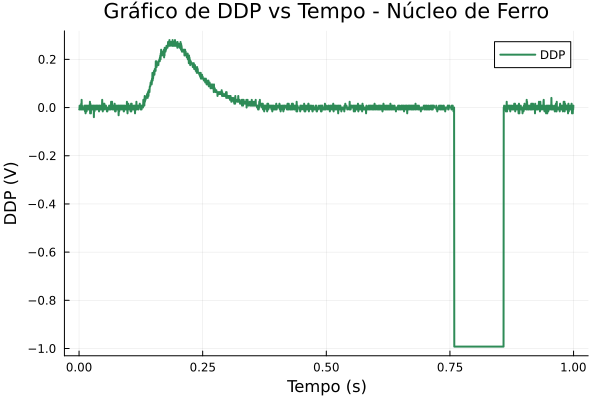
\includegraphics[width=1.0\linewidth]{figuras/grafico_dados3_F0007CH1.png}
\end{figure}

\begin{figure}[H]
    \centering
    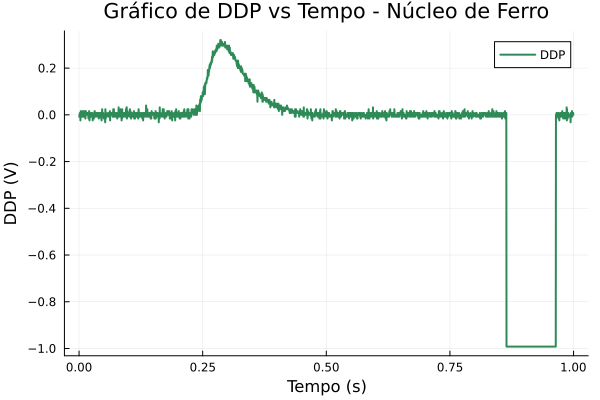
\includegraphics[width=1.0\linewidth]{figuras/grafico_dados3_F0008CH1.png}
\end{figure}

\begin{figure}[H]
    \centering
    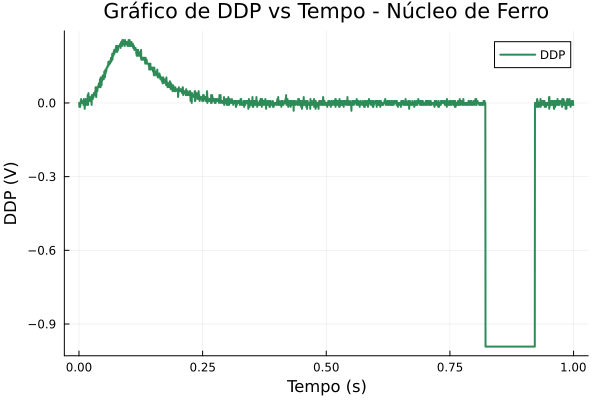
\includegraphics[width=1.0\linewidth]{figuras/grafico_dados3_F0009CH1.png}
\end{figure}

\begin{figure}[H]
    \centering
    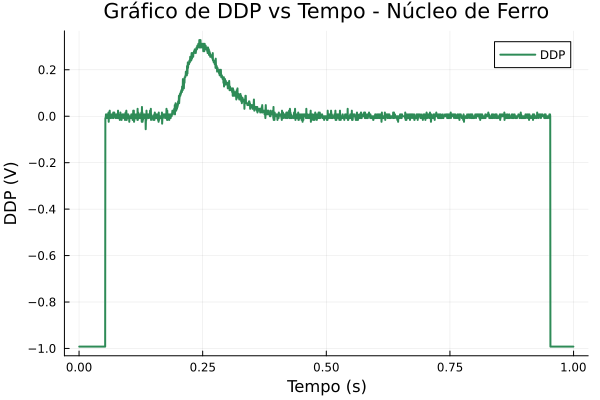
\includegraphics[width=1.0\linewidth]{figuras/grafico_dados3_F0010CH1.png}
\end{figure}

\begin{figure}[H]
    \centering
    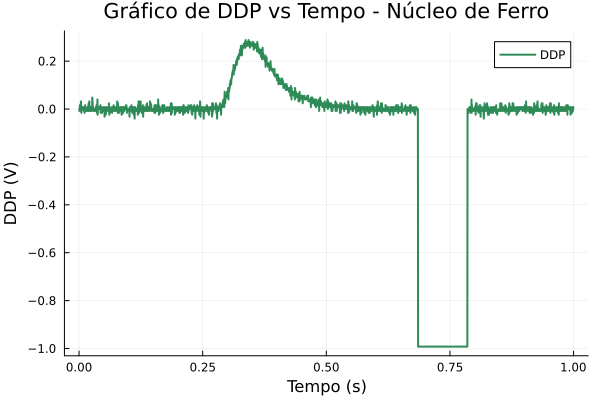
\includegraphics[width=1.0\linewidth]{figuras/grafico_dados3_F0011CH1.png}
\end{figure}

\begin{figure}[H]
    \centering
    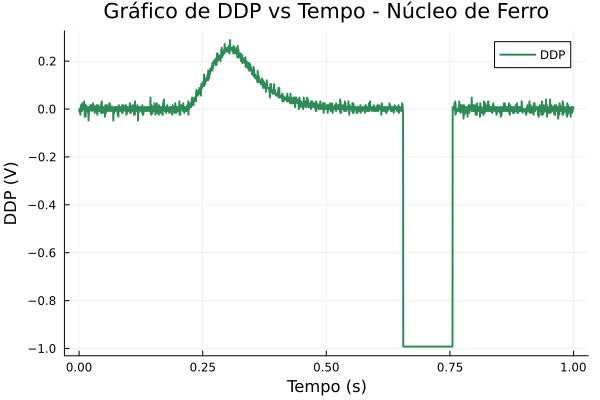
\includegraphics[width=1.0\linewidth]{figuras/grafico_dados3_F0012CH1.png}
\end{figure}

\end{multicols}
\end{center}



\end{document}